\documentclass[12pt,a4paper]{article}
\usepackage[utf8]{inputenc}
\usepackage[T1]{fontenc}
\usepackage{amsmath}
\usepackage{amssymb}
\usepackage{graphicx}
\usepackage{float}
\author{Mirco Huber}
\title{Grundlagen Sensorik}
\begin{document}
	\maketitle
	\newpage
	\section{Key Tageaways}
	\subsection{11.05.2023}
	Themen waren X-318: Gehäuse, Print, Sensoranschlüsse und Ladebuchse im Zusammenhang mit dem Schindler-BLE-X-318 (Project Ethiopian Fox). Weiter wurde die Ablage von Dateien in PDM angeschaut. Zu Letzt wurden FEM-Themen angeschnitten.
	\subsubsection{Solidworks / PDM}
	Dateien müssen in PDM nicht zwingend einen sprechenden Dateinamen vorweisen, da mittels Suchkarten nach Dateieigenschaften (=Metadaten; frei wählbare Key-Value-Paare) gesucht werden kann. Für die Solidworks-Dateitypen \textit{Drawing}, \textit{Part} und \textit{Assebmly} wurden Vorlagen angelegt, in welchen einige dieser Metadaten-Keys wie beispielsweise die NAV-Artikelnummer bereits angelegt wurden.\\
	Werden neue Dateien angelegt, sind diese bis zum ersten Einchecken nur lokal verfügbar.\\
	Dateien können nur ausgecheckt werden, wenn diese im Workflow in einem bearbeitbaren Modus (Bagatelländerung \& in Bearbeitung) sind.\\
	Auschecken bedeutet, dass man exklusives Schreibrecht auf die Datei hat. Die Änderungen stehen anderen erst zu Verfügung, wenn diese eingecheckt werden.\\
	Mittels \textit{Holen} wird die lokale Kopie einer Datei mit dem aktuellsten Stand der Datei auf dem PDM-Server überschrieben. Das Schreibrecht wird nicht benötigt und somit auch nicht eingefordert. Die Datei bleibt entsprechend im jeweiligen Workflow-Status eingecheckt.
	\subsubsection{FEM}
	Durch Verwendung von kurvengestützten Netzen kann die Effizienz der Simulation erhöht werden, da nur gewisse Ausschnitte des Parts in feiner Auslösung gerechnet werden müssen. Weiter lohnt es sich, das Part (sofern es Symmetrien aufweist) zu zerlegen. Features, welche keinen (grossen) Beitrag zur Festigkeit/Steifigkeit liefern wie beispielsweise Fasen sollten (besonders in einer Trial and Error Phase) für die Simulation unterdrückt werden.\\
	Die Rahmenbedingungen haben einen starken Einfluss auf die Resultate der FEM-Studie. Daher sollten diese so realitätsnahe wie möglich gesetzt werden. Einem Dehnungssensor sollte beispielsweise eine Verschiebung vorgeschrieben werden, während bei Kraftsensoren über externe Lasten eine physikalische Kraft aufgetragen werden kann. \\
	Studien können mittels Rechtsklick auf dem Studientab in der Fussleiste des Fensters einfach kopiert werden. Durch diese Kopien kann der Einfluss von veränderten Lasten gut visualisiert werden: Vorhanden Studie kopieren, Einspannungen und/oder Lasten ändern, BEIDE Studien ausführen, in der Navigationsliste oben \textit{Resultate vergleichen} wählen. Dadurch werden die Ergebnisse der Studien in zwei Fenstern nebeneinander in der jeweils identischen Perspektive angezeigt.\\
	Selbige Prozedur kann verwendet werden, um den Einfluss neuer Features am Part zu analysieren. Wenn eine Studie kopiert wird, kann im Dialog eine andere Konfiguration des Parts gewählt werden.\\
	Hauptvorteil dieser Prozedur ist, dass dank Kopieren der Studien Dinge wie Vernetzung, gewisse Einspannungen oder Lasten eins zu eins übernommen werde.
	\section{Sensoren}
	Im folgenden wird das Thema Sensorik, wie es bei X-Sensors AG verwendet wird, eingeführt.\\
	\textbf{Definition: \textit{Sensor}.}\newline
	Ein Sensor ist ein Bauteil, das eine physikalische Grösse in eine elektrische übersetzt.
	Grundsätzlich fertigt die Firma X-Sensors AG zwei Sorten von Sensoren: Dehnungs- und Kraftsensoren. Während Kraftsensoren direkt in den Kraftfluss eingebaut werden, werden Dehnungssensoren an die belasteten Strukturen angebracht und detektieren deren Verformung.
	\begin{figure}[H]
		\centering
		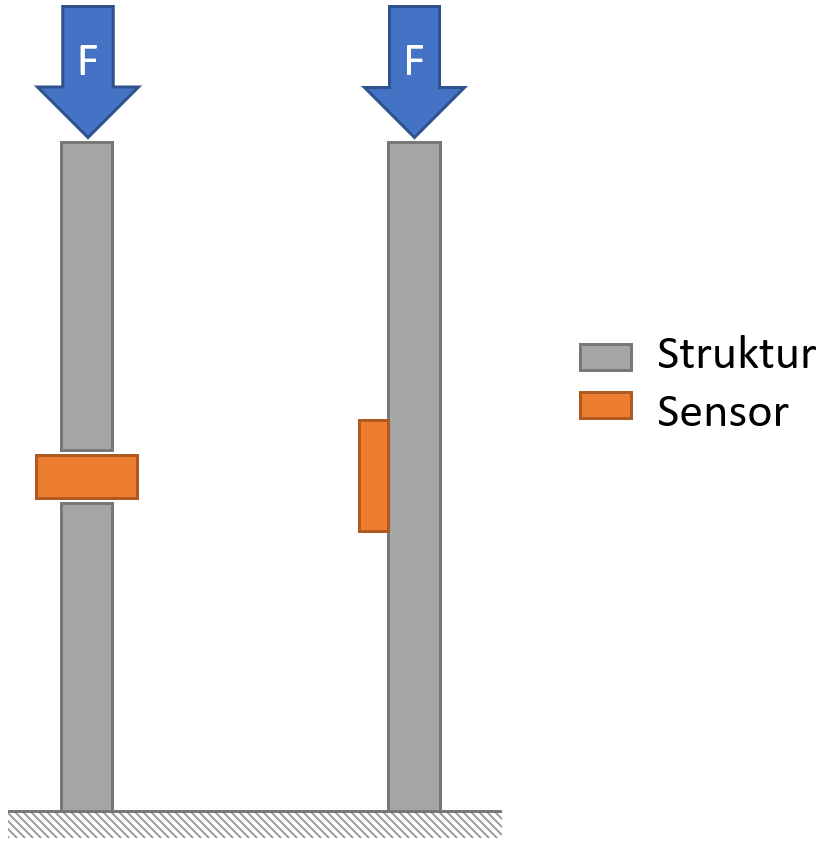
\includegraphics[width=.5\linewidth]{imgs/screenshot001}
		\caption{links: Kraftsensor, rechts: Dehnungssensor}
		\label{fig:screenshot001}
	\end{figure}\noindent
	Die Übersetzung der Dehnung respektive der Kraft in ein elektrisches Signal wird mittels DMS realisiert. DMS weisen einen nominalen elektrischen Wiederstand im Bereich von 100...1000 $\Omega$ auf. Dieser ändert sich, wenn der DMS gedehnt oder gestaucht wird. Der Zusammenhang zwischen Dehnung und Widerstandsänderung ist (innerhalb des zulässigen Bereichs) linear:
	\begin{equation}
		\frac{\Delta R}{R} = \epsilon \cdot k
	\end{equation}
	Mit: R: nominaler Widerstand [$\Omega$] des (unverformten) DMS, ${\Delta R}$ durch die Dehnung verursachte Widerstandsänderung [$\Omega$] des DMS, $\epsilon$: Dehnung [-], $k$: DMS-spezifische Proportionalitätskonstante a.k.a \textit{k-Faktor}

\end{document}